\documentclass[a4paper]{article}
\setlength{\oddsidemargin}{-0.7cm}
\setlength{\topmargin}{-1.5cm}
\setlength{\textwidth}{16.5cm}
\setlength{\textheight}{24cm}

\usepackage{amsmath}
\usepackage{graphics}

\newcommand{\ex}[1]{E[ #1 ]}
\newcommand{\xb}{\bar{\bf x}}
\newcommand{\sgm}{\sigma^2({\bf x})}
\newcommand{\ess}{{\cal S}({\bf x})}

\title{Unbiased Estimator for Fourth Moments}
\author{Synge Todo \\
  {\it Department of Physics, University of Tokyo, Tokyo 113-0033, Japan}}

\begin{document}
\maketitle

\section{Hybrids}
Before considering unbiased estimator for the fourth moments, we introduce more hybrids moments in addition to Online Appendix~M of Ref.~\cite{Klements2009}.
\begin{align}
  \begin{split}
    \ex{x_1 x_2 \xb^2} =& \frac{1}{n^2} \ex{x_1 x_2 (\sum_{i=1}^n x_i)^2} \\
    =& \frac{1}{n^2} \ex{x_1 x_2 (x_1^2 + x_2^2 + \sum_{i=3}^n x_i^2 + 2 x_1 x_2 + 2 x_1 (\sum_{i=3}^n x_i) + 2 x_2 (\sum_{i=3}^n x_i) + \sum_{i=3}^n\sum_{j=i+1}^n x_i x_j)} \\
    =& \frac{2}{n^2} \ex{x_1^3 x_2} + \frac{n-2}{n^2} \ex{x_1 x_2 x_3^2} + \frac{2}{n^2} \ex{x_1^2 x_2^2} + \frac{4(n-2)}{n^2} \ex{x_1^2 x_2 x_3} \\ &+ \frac{(n-2)(n-3)}{n^2} \ex{x_1 x_2 x_3 x_4} \\
    =& \frac{2}{n^2} (\ess + 3 \sgm \mu + \mu^3) \mu + \frac{5(n-2)}{n^2} (\sgm + \mu^2) \mu^2 + \frac{2}{n^2} (\sgm^2+\mu^2)^2 \\ &+ \frac{(n-2)(n-3)}{n^2} \mu^4 \\
    =& \frac{2}{n^2} \ess \mu + \frac{5}{n} \sgm \mu^2 + \frac{2}{n^2} \sigma^4 + \mu^4
  \end{split} \\
  \begin{split}
    \ex{x_1^2 x_2 \xb} =& \frac{1}{n} \ex{x_1^2 x_2 (\sum_{i=1}^n x_i)} \\
    =& \frac{1}{n} \ex{x_1^3 x_2 + x_1^2 x_2^2 + (n-2) x_1^2 x_2 x_3} \\
    =& \frac{1}{n} (\ess + 3 \sgm \mu + \mu^3) \mu + \frac{1}{n} (\sgm + \mu^2)^2 + \frac{n-2}{n} (\sgm + \mu^2) \mu^2 \\
    =& \frac{1}{n} \ess \mu + \frac{(n+3)}{n} \sgm \mu^2 + \frac{1}{n} \sigma^4 + \mu^4.
  \end{split}
\end{align}

\section{Square of variance, $\sigma_{\xb}^4({\bf x})$}

Expression for square of variance, $\sigma_{\xb}^4({\bf x})$, given on p.~9 in Online Appendix~M of Ref.~\cite{Klements2009} is not correct.  The correct expression is
\begin{align}
  \begin{split}
    \sigma_{\xb}^4({\bf x}) =& \ex{(x_i-\xb)^2(x_j-\xb)^2} \\
    =& \ex{\frac{1}{n}\sum(x_i-\xb)^2\cdot\frac{1}{n}\sum(x_j-\xb)^2} \\
    =& \frac{1}{n^2} \ex{\sum_i \sum_j (x_i-\xb)^2(x_j-\xb)^2} \\
    =& \frac{1}{n^2} \ex{\sum_i (x_i-\xb)^4} + \frac{1}{n^2} \ex{\sum_i \sum_{j\ne i} (x_i-\xb)^2(x_j-\xb)^2} \\
    =& \frac{1}{n} \ex{(x_1-\xb)^4} + \frac{n-1}{n} \ex{(x_1-\xb)^2(x_2-\xb)^2} \\
    =& \frac{1}{n} \ex{(x_1-\xb)^4} + \frac{n-1}{n} \ex{x_1^2 x_2^2 - 4 x_1^2 x_2 \xb + 2x_1^2 \xb^2 + 4 x_1 x_2 \xb^2 - 4 x_1 \xb^3 + \xb^4} \\
    =& \frac{1}{n} {\cal K_{\xb}(\bf x)}
    + \frac{n-1}{n} (\sgm + \mu^2)^2 \\
    &- \frac{4(n-1)}{n} \Big[ \frac{1}{n} \ess \mu + \frac{(n+3)}{n} \sgm \mu^2 + \frac{1}{n} \sigma^4 + \mu^4 \Big] \\
    &+ \frac{2(n-1)}{n} \Big[ \frac{1}{n^2} {\cal K}({\bf x}) + \frac{2(n+1)}{n^2} \ess \mu + \frac{n+5}{n} \sgm \mu^2 + \frac{n-1}{n^2} \sigma^4 + \mu^4 \Big] \\
    &+ \frac{4(n-1)}{n} \Big[ \frac{2}{n^2} \ess \mu + \frac{5}{n} \sgm \mu^2 + \frac{2}{n^2} \sigma^4 + \mu^4\Big] \\
    &- \frac{4(n-1)}{n} \Big[ \frac{1}{n^3} {\cal K}({\bf x}) + \frac{4}{n^2} \ess \mu + \frac{6}{n} \sgm \mu^2 + \frac{3(n-1)}{n^3} \sigma^4 + \mu^4 \Big] \\
    &+ \frac{n-1}{n} \Big[ \frac{1}{n^3} {\cal K}({\bf x}) + \frac{4}{n^2} \ess \mu + \frac{6}{n} \sgm \mu^2 + \frac{3(n-1)}{n^3} \sigma^4 + \mu^4 \Big] \\
    =& \frac{1}{n} {\cal K_{\xb}(\bf x)} + \frac{(n-1)(2n-3)}{n^4} {\cal K}({\bf x})
    + \frac{(n-1)(n^3-2n^2-3n+9)}{n^4} \sigma^4({\bf x}) \\
    =& \frac{n-1}{n^3} \Big[ (n-1) {\cal K}({\bf x}) + (n^2-2n+3) \sigma^4({\bf x}) \Big].
  \end{split}
  \label{eqn:square_of_variance}
\end{align}
In the last line in Eq.~(\ref{eqn:square_of_variance}), we use the expression for the fourth sample central moment:
\begin{align}
  \begin{split}
    {\cal K_{\xb}(\bf x)} = \ex{(x_i-\xb)^4} = \frac{n-1}{n^3} \Big[ (n^2-3n+3) {\cal K}({\bf x}) + (6n-9)\sigma^4({\bf x}) \Big],
  \end{split}
  \label{eqn:fourth_sample_central_moment}
\end{align}
which is given on p.~8 in Online Appendix~M of Ref.~\cite{Klements2009}.

\section{Unbiased estimator for $\sigma^4({\bf x})$, ${\cal K}({\bf x})$, and fourth cumulant}

By solving Eqs.~(\ref{eqn:square_of_variance}) and (\ref{eqn:fourth_sample_central_moment}), we obtain the unbiased estimators for the square of the variance, the fourth central moment, and the fourth cumulant as
\begin{align}
  \begin{split}
    \sigma^4({\bf x}) = \frac{n}{(n-1)(n-2)(n-3)} \Big[ (n^2-3n+3) \sigma_{\xb}^4({\bf x}) - (n-1) {\cal K_{\xb}(\bf x)} \Big]
  \end{split} \\
  \begin{split}
    {\cal K}({\bf x}) = \frac{n}{(n-1)(n-2)(n-3)} \Big[ (n^2-2n+3) {\cal K_{\xb}(\bf x)} - (6n-9) \sigma_{\xb}^4({\bf x}) \Big]
  \end{split} \\
  \begin{split}
    \kappa_4({\bf x}) = {\cal K}({\bf x}) - 3 \sigma^4({\bf x})
    = \frac{n^2}{(n-1)(n-2)(n-3)} \Big[ (n+1) {\cal K_{\xb}(\bf x)} - 3(n-1) \sigma_{\xb}^4({\bf x}) \Big],
  \end{split}
\end{align}
respectively.

\section{Numerical tests}

We test numerically the above expressions for the Bernoulli distribution ${\cal B}(p=3/4)$ and the normal distribution ${\cal N}(\mu=2,\sigma=3/2)$. We evaluate Eqs.~(1)--(7) for the sample size $n=4,8,16,32,\cdots,1024$. For each sample size, we take the average over 65536 sample sets and estimate the error bar. The results are shown in Figs.~1--7.

\bibliographystyle{naturemag}
\bibliography{fourth-moment}

\clearpage

\begin{figure}
  \begin{center}
    \resizebox{0.47\textwidth}{!}{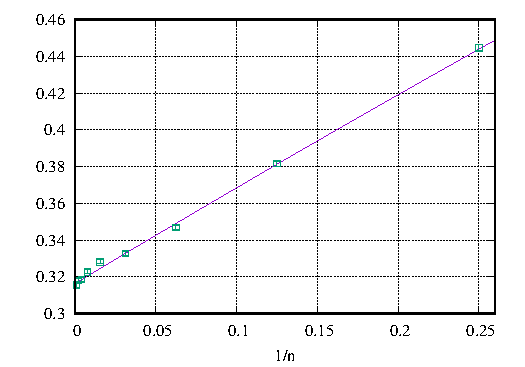
\includegraphics{plot-eq1-b.pdf}}
    \resizebox{0.47\textwidth}{!}{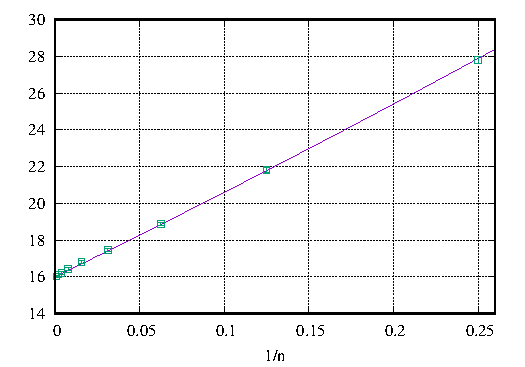
\includegraphics{plot-eq1-n.pdf}}
  \end{center}
  \caption{Sample-size dependence of $\ex{x_1 x_2 \xb^2}$ for the Bernoulli distribution ${\cal B}(p=3/4)$ (left) and the normal distribution ${\cal N}(\mu=2,\sigma=3/2)$ (right). The green squares denotes the numerical results and the purple line denotes Eq.~(1) calculated by using the exact moments.}
\end{figure}

\begin{figure}
  \begin{center}
    \resizebox{0.47\textwidth}{!}{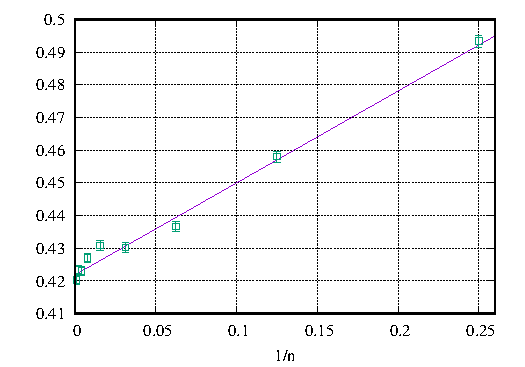
\includegraphics{plot-eq2-b.pdf}}
    \resizebox{0.47\textwidth}{!}{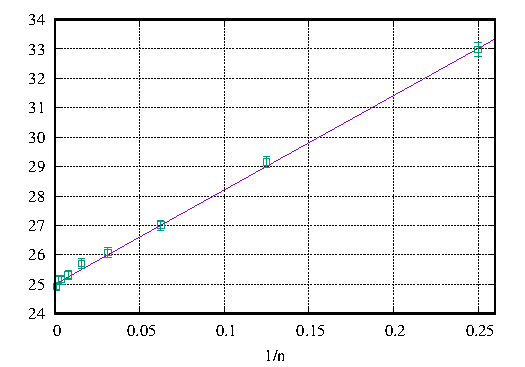
\includegraphics{plot-eq2-n.pdf}}
  \end{center}
  \caption{Sample-size dependence of $\ex{x_1^2 x_2 \xb}$ for the Bernoulli distribution ${\cal B}(p=3/4)$ (left) and the normal distribution ${\cal N}(\mu=2,\sigma=3/2)$ (right). The green squares denotes the numerical results and the purple line denotes Eq.~(2) calculated by using the exact moments.}
\end{figure}

\begin{figure}
  \begin{center}
    \resizebox{0.47\textwidth}{!}{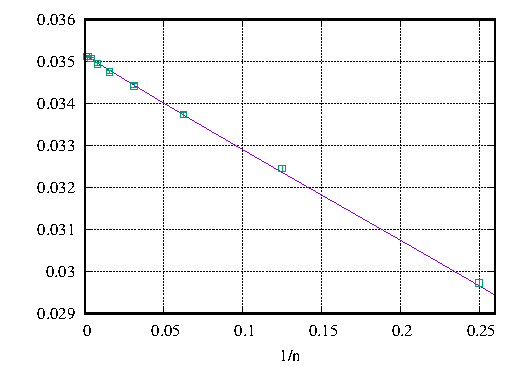
\includegraphics{plot-eq3-b.pdf}}
    \resizebox{0.47\textwidth}{!}{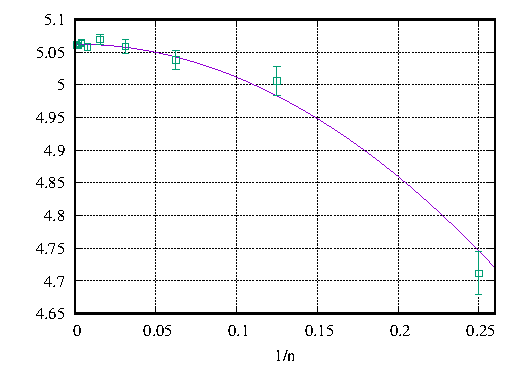
\includegraphics{plot-eq3-n.pdf}}
  \end{center}
  \caption{Sample-size dependence of $\sigma_{\xb}^4({\bf x})$ for the Bernoulli distribution ${\cal B}(p=3/4)$ (left) and the normal distribution ${\cal N}(\mu=2,\sigma=3/2)$ (right). The green squares denotes the numerical results and the purple line denotes Eq.~(3) calculated by using the exact moments.}
\end{figure}

\begin{figure}
  \begin{center}
    \resizebox{0.47\textwidth}{!}{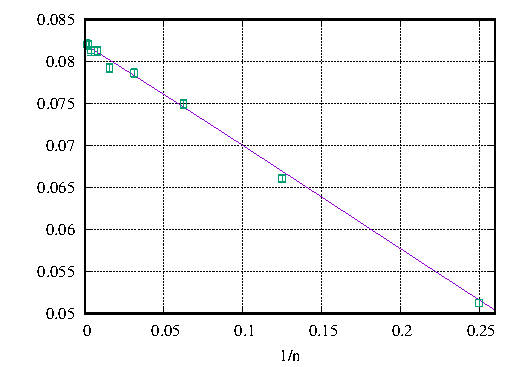
\includegraphics{plot-eq4-b.pdf}}
    \resizebox{0.47\textwidth}{!}{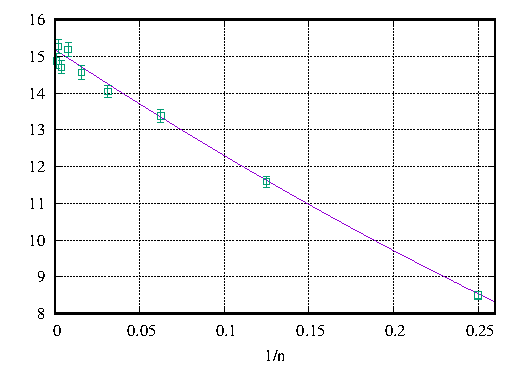
\includegraphics{plot-eq4-n.pdf}}
  \end{center}
  \caption{Sample-size dependence of ${\cal K_{\xb}(\bf x)}$ for the Bernoulli distribution ${\cal B}(p=3/4)$ (left) and the normal distribution ${\cal N}(\mu=2,\sigma=3/2)$ (right). The green squares denotes the numerical results and the purple line denotes Eq.~(4) calculated by using the exact moments.}
\end{figure}

\begin{figure}
  \begin{center}
    \resizebox{0.47\textwidth}{!}{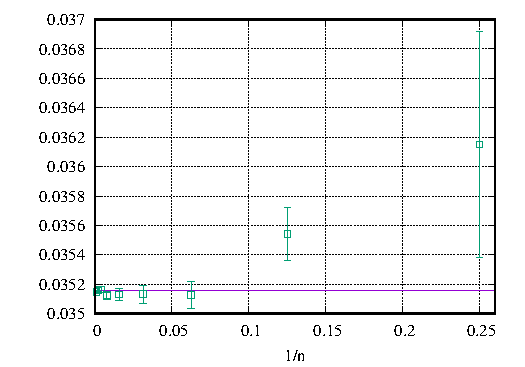
\includegraphics{plot-eq5-b.pdf}}
    \resizebox{0.47\textwidth}{!}{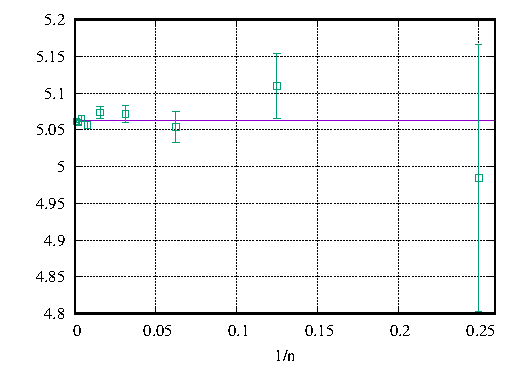
\includegraphics{plot-eq5-n.pdf}}
  \end{center}
  \caption{Results for the square of the variance, $\sigma^4({\bf x})$, by using the unbiased estimator~(5) for the Bernoulli distribution ${\cal B}(p=3/4)$ (left) and the normal distribution ${\cal N}(\mu=2,\sigma=3/2)$ (right). The green squares denotes the numerical results and the purple line denotes the exact value.}
\end{figure}

\begin{figure}
  \begin{center}
    \resizebox{0.47\textwidth}{!}{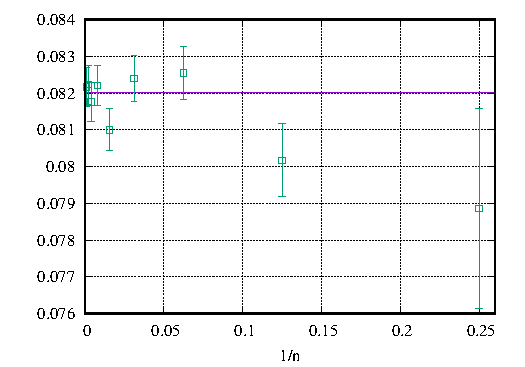
\includegraphics{plot-eq6-b.pdf}}
    \resizebox{0.47\textwidth}{!}{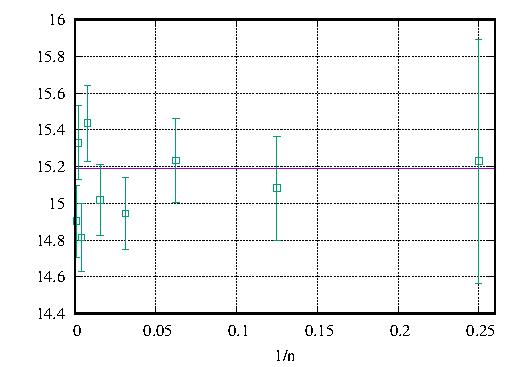
\includegraphics{plot-eq6-n.pdf}}
  \end{center}
  \caption{Results for the fourth central moment, ${\cal K}({\bf x})$, by using the unbiased estimator~(6) for the Bernoulli distribution ${\cal B}(p=3/4)$ (left) and the normal distribution ${\cal N}(\mu=2,\sigma=3/2)$ (right). The green squares denotes the numerical results and the purple line denotes the exact value.}
\end{figure}

\begin{figure}
  \begin{center}
    \resizebox{0.47\textwidth}{!}{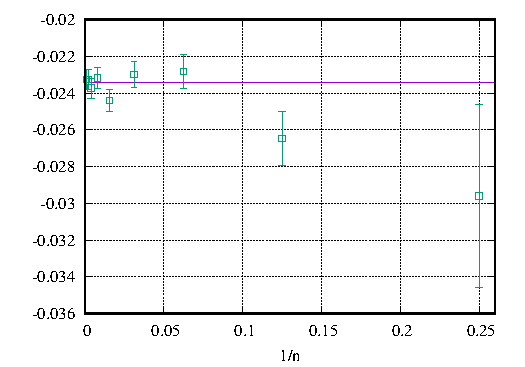
\includegraphics{plot-eq7-b.pdf}}
    \resizebox{0.47\textwidth}{!}{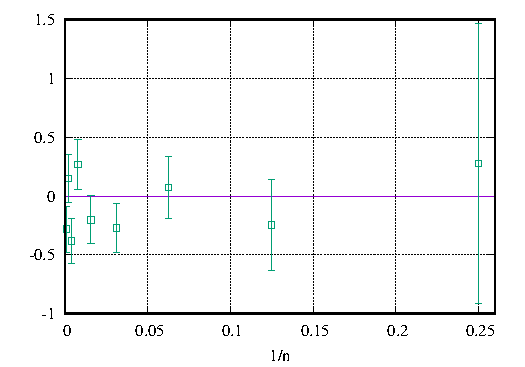
\includegraphics{plot-eq7-n.pdf}}
  \end{center}
  \caption{Results for the fourth cumulant, $\kappa_4({\bf x})$, by using the unbiased estimator~(6) for the Bernoulli distribution ${\cal B}(p=3/4)$ (left) and the normal distribution ${\cal N}(\mu=2,\sigma=3/2)$ (right). The green squares denotes the numerical results and the purple line denotes the exact value.}
\end{figure}

\end{document}
